\documentclass{article}
\usepackage{tikz}
\usepackage{amsmath}
\usetikzlibrary{arrows.meta}

\begin{document}

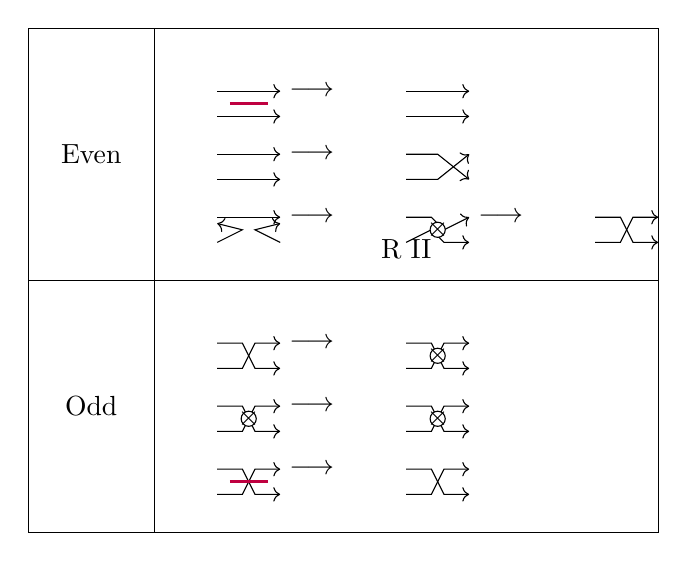
\begin{tikzpicture}[scale=0.8]
% Grid and labels
\draw (0,0) rectangle (10,8);
\draw (0,4) -- (10,4);
\draw (2,0) -- (2,8);
\node at (1,6) {Even};
\node at (1,2) {Odd};
\node at (6,4.5) {R II};

% Even section, first row
\begin{scope}[shift={(3,7)}]
  \draw[->] (0,0) -- (1,0);
  \draw[->] (0,-0.4) -- (1,-0.4);
  \draw[purple] (0.5,-0.2) -- (0.5,-0.2);
  \draw[purple, line width=1pt] (0.2,-0.2) -- (0.8,-0.2);
\end{scope}
\node at (4.5,7) {$\longrightarrow$};
\begin{scope}[shift={(6,7)}]
  \draw[->] (0,0) -- (1,0);
  \draw[->] (0,-0.4) -- (1,-0.4);
\end{scope}

% Even section, second row
\begin{scope}[shift={(3,6)}]
  \draw[->] (0,0) -- (1,0);
  \draw[->] (0,-0.4) -- (1,-0.4);
\end{scope}
\node at (4.5,6) {$\longrightarrow$};
\begin{scope}[shift={(6,6)}]
  \draw[->] (0,0) -- (0.5,0) -- (1,-0.4);
  \draw[->] (0,-0.4) -- (0.5,-0.4) -- (1,0);
\end{scope}

% Even section, third row
\begin{scope}[shift={(3,5)}]
  \draw[->] (0,0) -- (1,0);
  \draw[->] (0,-0.4) -- (0.4,-0.2) -- (0,-0.1);
  \draw[->] (1,-0.4) -- (0.6,-0.2) -- (1,-0.1);
\end{scope}
\node at (4.5,5) {$\longrightarrow$};
\begin{scope}[shift={(6,5)}]
  \draw[->] (0,0) -- (0.4,0) -- (0.6,-0.2) -- (1,0);
  \draw[->] (0,-0.4) -- (0.4,-0.2) -- (0.6,-0.4) -- (1,-0.4);
  \draw[purple, line width=1pt] (0.5,-0.3) -- (0.5,-0.1);
  \fill[white] (0.5,-0.2) circle (0.12);
  \draw (0.5,-0.2) circle (0.12);
  \node at (0.5,-0.2) {$\times$};
\end{scope}
\node at (7.5,5) {$\longrightarrow$};
\begin{scope}[shift={(9,5)}]
  \draw[->] (0,0) -- (0.4,0) -- (0.6,-0.4) -- (1,-0.4);
  \draw[->] (0,-0.4) -- (0.4,-0.4) -- (0.6,0) -- (1,0);
\end{scope}

% Odd section, first row
\begin{scope}[shift={(3,3)}]
  \draw[->] (0,0) -- (0.4,0) -- (0.6,-0.4) -- (1,-0.4);
  \draw[->] (0,-0.4) -- (0.4,-0.4) -- (0.6,0) -- (1,0);
\end{scope}
\node at (4.5,3) {$\longrightarrow$};
\begin{scope}[shift={(6,3)}]
  \draw[->] (0,0) -- (0.4,0) -- (0.6,-0.4) -- (1,-0.4);
  \draw[->] (0,-0.4) -- (0.4,-0.4) -- (0.6,0) -- (1,0);
  \fill[white] (0.5,-0.2) circle (0.12);
  \draw (0.5,-0.2) circle (0.12);
  \node at (0.5,-0.2) {$\times$};
\end{scope}

% Odd section, second row
\begin{scope}[shift={(3,2)}]
  \draw[->] (0,0) -- (0.4,0) -- (0.6,-0.4) -- (1,-0.4);
  \draw[->] (0,-0.4) -- (0.4,-0.4) -- (0.6,0) -- (1,0);
  \fill[white] (0.5,-0.2) circle (0.12);
  \draw (0.5,-0.2) circle (0.12);
  \node at (0.5,-0.2) {$\times$};
\end{scope}
\node at (4.5,2) {$\longrightarrow$};
\begin{scope}[shift={(6,2)}]
  \draw[->] (0,0) -- (0.4,0) -- (0.6,-0.4) -- (1,-0.4);
  \draw[->] (0,-0.4) -- (0.4,-0.4) -- (0.6,0) -- (1,0);
  \fill[white] (0.5,-0.2) circle (0.12);
  \draw (0.5,-0.2) circle (0.12);
  \node at (0.5,-0.2) {$\times$};
\end{scope}

% Odd section, third row
\begin{scope}[shift={(3,1)}]
  \draw[->] (0,0) -- (0.4,0) -- (0.6,-0.4) -- (1,-0.4);
  \draw[->] (0,-0.4) -- (0.4,-0.4) -- (0.6,0) -- (1,0);
  \draw[purple, line width=1pt] (0.2,-0.2) -- (0.8,-0.2);
\end{scope}
\node at (4.5,1) {$\longrightarrow$};
\begin{scope}[shift={(6,1)}]
  \draw[->] (0,0) -- (0.4,0) -- (0.6,-0.4) -- (1,-0.4);
  \draw[->] (0,-0.4) -- (0.4,-0.4) -- (0.6,0) -- (1,0);
\end{scope}

\end{tikzpicture}

\end{document}